\documentclass[sigplan,screen]{acmart}
% \documentclass[manuscript,screen,review]{acmart}

\setcopyright{none}
\settopmatter{printacmref=false}
\renewcommand\footnotetextcopyrightpermission[1]{}


%\setcopyright{acmcopyright}
%\copyrightyear{2018}
%\acmYear{2018}
%\acmDOI{XXXXXXX.XXXXXXX}

%\acmConference[Conference acronym 'XX]{Make sure to enter the correct
%  conference title from your rights confirmation emai}{June 03--05,
%  2018}{Woodstock, NY}

%\acmBooktitle{Woodstock '18: ACM Symposium on Neural Gaze Detection,
%  June 03--05, 2018, Woodstock, NY} 
%\acmPrice{15.00}
%\acmISBN{978-1-4503-XXXX-X/18/06}

%%\acmSubmissionID{123-A56-BU3}

%%\citestyle{acmauthoryear}


\begin{document}

\title{Cloudmesh-cc: Hybrid analytics computation management}

\author{Gregor von Laszewski}
\email{laszewski@gmail.com}
\orcid{0000-0001-9558-179X}
\authornote{Corresponding author}
\affiliation{%
  \institution{University of Virginia}
  \streetaddress{Biocomplexity Institute\\
Town Center Four\\
994 Research Park Boulevard}
  \city{Charlottesville}
  \state{VA}
  \postcode{22911}
  \country{USA}
}

\author{J.P. Fleischer}
\affiliation{%
  \institution{University of Virginia}
  \streetaddress{Biocomplexity Institute\\
Town Center Four\\
994 Research Park Boulevard}
  \city{Charlottesville}
  \state{VA}
  \postcode{22911}
  \country{USA}
}

\author{Geoffrey C. Fox}
\email{gcfexchange@gmail.com}
\affiliation{%
  \institution{University of Virginia}
  \streetaddress{Biocomplexity Institute\\
Town Center Four\\
994 Research Park Boulevard}
  \city{Charlottesville}
  \state{VA}
  \postcode{22911}
  \country{USA}
}

\renewcommand{\shortauthors}{von Laszewski, et al.}

\begin{abstract}

  TBD

 \end{abstract}

  
\begin{CCSXML}
<ccs2012>
<concept>
<concept_id>10010520.10010521.10010537</concept_id>
<concept_desc>Computer systems organization~Distributed architectures</concept_desc>
<concept_significance>500</concept_significance>
</concept>
<concept>
<concept_id>10010520.10010521.10010537.10003100</concept_id>
<concept_desc>Computer systems organization~Cloud computing</concept_desc>
<concept_significance>500</concept_significance>
</concept>
<concept>
<concept_id>10011007.10010940.10010971.10011120</concept_id>
<concept_desc>Software and its engineering~Distributed systems organizing principles</concept_desc>
<concept_significance>500</concept_significance>
</concept>
</ccs2012>
\end{CCSXML}

\ccsdesc[500]{Computer systems organization~Distributed architectures}
\ccsdesc[500]{Computer systems organization~Cloud computing}
\ccsdesc[500]{Software and its engineering~Distributed systems organizing principles}

\keywords{high performance computing, batch queue, service}


  
\keywords{datasets, neural networks, gaze detection, text tagging}

%\received{20 February 2007}
%\received[revised]{12 March 2009}
%\received[accepted]{5 June 2009}

% set page numbers
\settopmatter{printfolios=true}

\maketitle


\begin{CCSXML}
<ccs2012>
<concept>
<concept_id>10010520.10010521.10010537</concept_id>
<concept_desc>Computer systems organization~Distributed architectures</concept_desc>
<concept_significance>500</concept_significance>
</concept>
<concept>
<concept_id>10010520.10010521.10010537.10003100</concept_id>
<concept_desc>Computer systems organization~Cloud computing</concept_desc>
<concept_significance>500</concept_significance>
</concept>
<concept>
<concept_id>10011007.10010940.10010971.10011120</concept_id>
<concept_desc>Software and its engineering~Distributed systems organizing principles</concept_desc>
<concept_significance>500</concept_significance>
</concept>
</ccs2012>
\end{CCSXML}

\ccsdesc[500]{Computer systems organization~Distributed architectures}
\ccsdesc[500]{Computer systems organization~Cloud computing}
\ccsdesc[500]{Software and its engineering~Distributed systems organizing principles}

\keywords{high performance computing, batch queue, service}



\section{Introduction}

\FILE{cc.tex}

\section{Introduction}

In this section we provide an introduction to or work while 
moving forward to motivate a 
Hybrid Reusable Computational Analytics Workflow
Management Framework.

\subsection{Reusable Computational Analytics}

{\em Reusable computational analytics} (RCA) focuses on  the creation of reusable programs, patterns, and services to conduct analytics tasks that are part of the scientific discovery process.  RCA service need varies widely and may include multi-scale hardware resources as well as multi-scale scientific applications. To utilize such services and their resources in a reusable way we need to have a mechanism to express them in an easy fashion that goes beyond just the definition in one programming language or framework, but allows the integration into many different programming languages and frameworks so that services that may be designed in one framework or language may be reusable in others.

\subsection{Reusable Multi-scale Algorithms}

In current scientific problems we encounter a rich set of applications that leverage a number of sophisticated methods that may require adaptations on multiple scales. The scales are influenced by their Domain size, accuracy and time requirement to solve them in sufficient manner. It is of advantage to provide reusable components that can be controlled by parameters to simplify reuse.

\subsection{Hybrid Cloud and Compute Resources and Serices}

As we deal with multi-scale algorithms not every analytics task needs to be conducted on a High Performance Computer (HPC). This is especially the case with the advent of GPUs in the desktop which we termed in the authors termed in past with {\em desktop supercomputing}. Also the availability of cloud computers and hyper-scale data centers play a significant role in today's analytics processes. This not only includes the use compute resources, but also services that are these days offered by cloud service providers. A well known example for this is natural language processing.

\subsection{Reusable and Adaptable HPC and Cloud Service Workflows}

High-performance computing (HPC) has been, for decades, a very important tool
for science. Scientific tasks can leverage the processing power of
a supercomputer so they can run at previously unobtainable high speeds
or utilize specialized hardware for acceleration that otherwise are not
available to the user. HPC can be used for analytic programs that
leverage machine learning applied to large data sets to, for example,
predict future values or to model current states. For such
high-complexity projects, there are often multiple complex programs that
may be running repeatedly in either competition or cooperation.
Leveraging computational GPUs, for instance, leads to several times higher
performance when applied to deep learning algorithms. With such
projects, program execution is submitted as a job to a typically remote
HPC center, where time is billed as node hours. Such projects must have
a service that lets the user manage and execute without supervision. We
have created a service that lets the user run jobs across multiple
platforms in a dynamic queue with visualization and data storage.

Similar aspects are available for cloud services that abstract the infrastructure needs and focus on the availability of services that can be integrated in concert with HPC, as well as the users local resources (for example a PC).




\section{Cloudmask Workflow}\label{cloudmask-workflow}

Cloudmesh cc comes with an example workflow that runs Cloudmask, which
is a program that develops a model to classify sections of satellite
images. Information regarding Cloudmask can be found at
\url{https://github.com/laszewsk/mlcommons/tree/main/benchmarks/cloudmask\#readme}

\subsection{Running the Cloudmask Workflow on
Rivanna}\label{running-the-cloudmask-workflow-on-rivanna}

To execute the workflow on UVA's HPC supercomputer, Rivanna, first
ensure that your UVA Computing ID is set with the following command,
replacing the X's with your ID:

\begin{verbatim}
me@mycomputer $ cms set username=XXXXXX
\end{verbatim}

Then, connect to the UVA Anywhere VPN and then download the satellite
data into your
\href{https://www.rc.virginia.edu/userinfo/storage/non-sensitive-data/\#scratch}{scratch}
directory on Rivanna:

\begin{verbatim}
me@mycomputer $ cms vpn connect
me@mycomputer $ ssh rivanna
rivanna $ cd /scratch/$USER
rivanna $ git clone https://github.com/laszewsk\
/mlcommons.git
rivanna $ cd mlcommons/benchmarks/cloudmask\
/target/rivanna
rivanna $ make data
# downloading the data will take a while.
rivanna $ exit
\end{verbatim}

Next, clone the \texttt{mlcommons} repository on your local machine and
run the workflow:

\begin{verbatim}
me@mycomputer $ cd ~/cm
me@mycomputer $ git clone https://github.com\
/laszewsk/mlcommons.git
me@mycomputer $ cd mlcommons
me@mycomputer $ pytest -v -x --capture=no \ 
benchmarks/cloudmask/target/rivanna/run_cloudmask\
_workflow.py
\end{verbatim}

The workflow iterates through the five GPUs available on Rivanna---
A100, V100, P100, RTX2080, and K80--- and runs the program three times
on each GPU. Each run trains the model with 10, 30, and 50 epochs for
benchmarking.

Upon completing a run, the logs and benchmarks of the program can be
found in the target folder:

\begin{verbatim}
me@mycomputer $ ssh rivanna
rivanna $ cd /scratch/$USER/mlcommons\
/benchmarks/cloudmask/target
\end{verbatim}

Additionally, the generated \texttt{.h5} model file can be found in the
home directory:

\begin{verbatim}
 rivanna $ cd ~/sciml_bench/outputs/slstr_cloud/
 \end{verbatim}

The program may take a while to run if the resources on Rivanna are
being used by other jobs.

\hypertarget{what-is-cloudmesh-cc}{%
\section{What Is Cloudmesh cc?}\label{what-is-cloudmesh-cc}}

Cloudmesh Compute Cluster (cc for short) is a repository of Python code
within the Cloudmesh suite that enables the creation of workflows. The
repository is compatible with Windows, macOS, and Linux.

Workflows are compilations of jobs to be run on nodes. These workflows
report information on the status of jobs as they are run, whether
locally or remotely. These jobs can be bash scripts, Python scripts,
Jupyter notebooks, or Slurm scripts. These types of jobs can be mixed
with one another in a single workflow.

The advantage that Cloudmesh cc provides is an interface to view the
progress of a workflow as it is being run in realtime. The workflow can
be monitored as a graph or a datatable. These interfaces report the
statuses of the jobs. Additionally, the order in which the jobs are run
can be specified, enabling prerequisite jobs and the segmentation of a
workflow.

Cloudmesh cc is bundled with pytests and examples that can be run on
your local machine or on HPC centers such as UVA's Rivanna supercomputer
(authentication is required for the latter). We encourage you to adapt
these tests to fit your HPC environment.

\section{MNIST Workflow}\label{mnist-workflow}

For this example we use UVA's Rivanna machine. Please adopt it to your
HPC machine.

We can test Rivanna's GPUs and benchmark their runtimes for running
several MNIST Python programs. These programs include machine learning
processing, convolutional neural network, long short-term memory,
recurrent neural network, and others. The programs can be found at
\url{https://github.com/cybertraining-dsc/reu2022/tree/main/code/deeplearning/mnist}

To run the MNIST remote workflow on Rivanna, first ensure that your UVA
computing ID is set with the following command:

\begin{verbatim}
cms set username=XXXXXX
\end{verbatim}

where the X's are substituted with your computing ID.

Then, issue commands:

\begin{verbatim}
cd ~/cm/cloudmesh-cc
pytest -v -x --capture=no examples/example_run_mnist_workflow_exec.py
\end{verbatim}

This program uses SLURM and a shell script to iterate through the
available GPUs on Rivanna, which are V100, A100, K80, P100, and RTX2080.

On a successful run, the output will be similar to the following:

\begin{verbatim}
+---------+----------+---------+---------+---------------------+
| Name    | Status   |    Time |     Sum | Start               |
|---------+----------+---------+---------+---------------------+
| v100    | ok       | 138.087 | 138.087 | 2022-09-29 18:15:45 |
| a100    | ok       | 106.046 | 106.046 | 2022-09-29 18:18:05 |
| k80     | ok       | 171.057 | 171.057 | 2022-09-29 18:19:52 |
| p100    | ok       | 202.055 | 202.055 | 2022-09-29 18:22:44 |
| rtx2080 | ok       | 138.048 | 138.048 | 2022-09-29 18:26:07 |
+---------+----------+---------+---------+---------------------+
\end{verbatim}

\FILE{quickstart.tex}

\section{Cloudmesh-cc Interfaces}

In this section we explain the various ways of interfacing with cloudmesh-cc.

It is important to note that we have a {\em commandline mode} that interfaces directly with the backends while not requiering a service. This includes an easy to use python API.

In addition we have used this API to implement a {\em service mode}, so we an stand up a REST service as well as a GUI that can ba accessed through a Web browser.
Please note that the service mode can also be access through te command line in a terminal. To distinguish how we operate cloudmesh-cc we use the term {\em mode} to deliniate it from a command that is entered ina terminal to query the status of the workflow.

We will now discuss tes interfaces in more detail and also showcase
hwo we can access them.


\subsection{Python API}

Cloudmesh-cc is implemented in Python. Extensive documentation is
available in GitHub and through GitHub action it is automatically
updated \cite{github-cloudmesh-cc}.  We distingush two main classes
that are easy to use. The first is a {\em Job class} that can adapted
to include new computational resource types for executing jobs. The
second is a {\em Workflow class} to ccordinate the execution of
multiple jobs. Selected methods of the Job class include are listed in
Figure~\ref{fig:code-job}. Important to note is that the code for the
scripts are all managed locally and a synchronization step is invoked
prior to one running the job to assure that the latest script and
code to be executed on the compute resource is available.

The most important part of using the Workflow Python API is showcased
in Figure~\ref{fig:code-job}, where we explain how easy it is to set up a workflow
with the Python API.

\begin{figure}[!h]
\begin{minted}[breaklines]{bash}
class Job:
   ...
   def clear():
      """Clear job progress."""
   def create(filename=None, script=None, exec=None):
      """Create a template for the script with progress."""
   def get_log(refresh=True):
      """Get the log of the job."""
   def get_pid(refresh=False):
      """Get the pid that the job is running within determined by the compute resource it is running on."""
   def get_progress(refresh=False):
       """Get the progress of the job from the compute resource."""
   def get_status(refresh=False):
       """Get the status of the job."""
   def kill():
       """Kill the job."""
   def run():
       """Run the job."""
   def sync():
       """Synchronise the current directory with the remote. Copies the shell script to the experiment directory and ensures that the file is copied with the sync command."""
   def watch(period=10):
       """Watch the job and check for changes in the given period."""
\end{minted}
\caption{Pseudo code for the Job class with selected methhods}
\label{fig:code-job}

\bigskip

\begin{minted}[breaklines]{bash}
class Workflow:
    ...
    def add_dependencies(dependency)
        """Add a job dependency to the workflow (and the graph)."""
    add_dependency(source, destination)
        """Add a job dependency to the workflow (and the graph)."""
    def add_job( ... ):
        """Add a job to the workflow with appropriate parameters."""
    def display(filename=None, name='workflow', first=True)
        """Show the graph of the workflow."""
    def job(name):
        """Return the details of a job within the workflow."""
    def load(filename, clear=True)
        """Load the workflow."""
    def remove_job(name, state=False)
        """Remove a particular job from the workflow."""
    def remove_workflow()
        """Delete workflow from the local file system."""
    def run_parallel( ... )
        """Run a workflow in a parallel fashion."""
    def run_topo(order=None, dryrun=False, show=True, filename=None)
        """Run the workflow in a topological order."""
    def save(filename=None):
        """Save the workflow."""
    def save_with_state(filename, stdout=False):
        """Save the workflow with state."""
    def sequential_order():
        """Return a list of the topological order of the workflow."""
    property table
        """Return a table of the workflow."""
    def update_progress(name):
        """Manually update the progress of a job according to its log file."""
    def update_status(name, status):
        """Manually update a job’s status."""
\end{minted}
\caption{Pseudo code for the Job class with selected methhods}
\label{fig:code-workflow}
\end{figure}


\begin{figure}[htb]
\begin{minted}[breaklines]{bash}
    w = Workflow(filename="workflow.yaml")
    # load a preexisting work=flow
    # w.load(filename="source.yaml") 
    # w.add(filename="source.yaml")
    
    # add jobs and dependencies explicitly
    w.add_job(name="fetch-data",
                command="hostname",
                host='supercomputer-a' # defined in .ssh
                label="{name}\nprogress={progress}",
                kind="local",
                status="ready",
                progress=0)
    w.add_job(name="compute", command="... TBD ...")
    w.add_job(name="analyze", command="... TBD ...")
    w.add_dependencies(
      dependency="start,fetch-data,compute,analyze"
    )
    w.run()
\end{minted}
\caption{Pseudo code for the Job class with selected methods}
\label{fig:code-workflow-example}

\bigskip

\begin{minted}[breaklines]{bash}
      cms cc workflow add [--name=NAME] [--job=JOB] ARGS...
      cms cc workflow add [--name=NAME] --filename=FILENAME
      cms cc workflow delete [--name=NAME] [--job=JOB]
      cms cc workflow list [--name=NAME] [--job=JOB]
      cms cc workflow run [--name=NAME] [--job=JOB] [--filename=FILENAME]
      cms cc workflow [--name=NAME] --dependencies=DEPENDENCIES
      cms cc workflow status --name=NAME [--output=OUTPUT]
      cms cc workflow graph --name=NAME
\end{minted}
\caption{Command line interface to the workflow in terminal mode}
\label{fig:code-workflow-commandline}

\bigskip

\begin{minted}[breaklines]{bash}
      cms cc start [-c] [--reload] [--host=HOST] [--port=PORT]
      cms cc stop
      cms cc status
      cms cc workflow service add [--name=NAME] FILENAME
      cms cc workflow service list [--name=NAME] [--job=JOB]
      cms cc workflow service add [--name=NAME] [--job=JOB] ARGS...
      cms cc workflow service run --name=NAME
\end{minted}
\caption{Command line interface to the workflow in service mode}
\label{fig:code-workflow-service-commandline}.

% \bigskip

{\centering
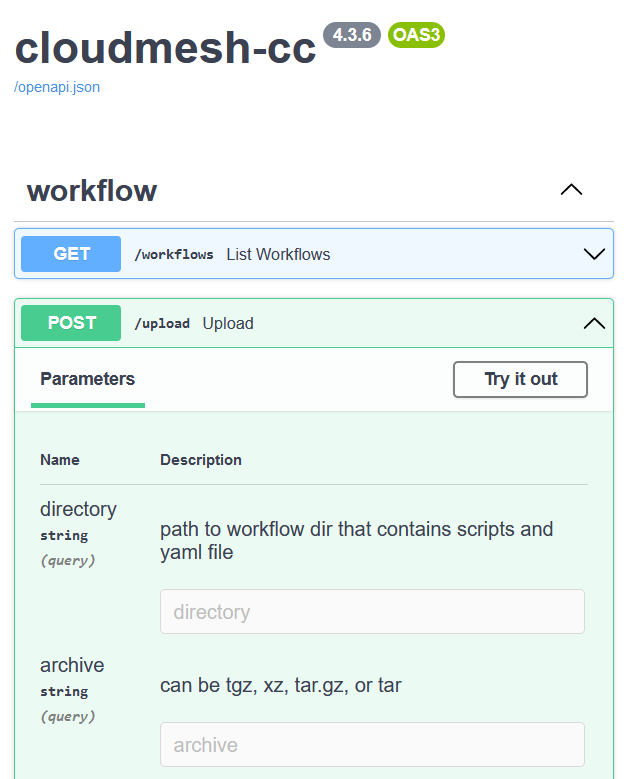
\includegraphics[width=0.52\columnwidth]{images/upload_api.png}
}
\caption{Browser API GUI for Cloudmesh Compute Cluster}

\label{fig:openapi}

\end{figure}


\subsection{Commandline Mode}

The commandline mode is an implementation that does not use a backend
service. It runs in the terminal until the workflow is completed. All
states of the jobs are managed on the compute service on which the job
is run and the status is replicated into the client on demand. This
allows easy reporting of the status through a table and a graph
display using client based rendering tools. The various commands to
interact with it on the commandline are shown in
Figure~\ref{fig:code-workflow-commandline}.


\subsection{Service Mode}

The Python API has ale been used to implement a REST service. To
easily interact with the REST service we have also added a couple of
conveneinet commannds one can issue from a terminal. They are listed
in Figure~\ref{fig:code-workflow-service-commandline}. It is clear for
these methods that starting stopping and getting the status of the
stevice is very easy, In contrast to the commandline mode this service
mode has an additional keyword {\em service} to intaract with the rest service.

Certainly one can also directly interact with the REST service API for
this service.  For ease of use we have exposed the interface thwough
an OpenAPI specification that is availeable to the user as shown in
Figure~\ref{fig:openapi}.



Thus other tools such as curl or other languages supporting url
requests can be used. A curl example to list the workflow
specifications uploaded to the service is

As we use a REST service, we can also easily upload the workflow
through a Python enabled REST call. We will use Python requests to
demonstrate this upload feature. To showcase the various ways to
access the service we focus on uploading a tar file that contains the workflow as well as the scripts or programs used in the workflow. The tar file is called {\em workflow.tar}

To also allow programming against the REST service in Python a Python
API similar to that pf the commanindline mode is
avalable. Figure~\ref{fig:code-workflow-rest-commandline} showcases
this API.

To implify interaction with the Rest service we create a special
RESTWorkflow class that is similar to the command module API but uses
instead the REST interface to the service rather then directly
communication with the command client API.

If the user wants to use instead just python requests he can do so as
follows, while we just showcase the program in
Figure~\ref{fig:code-workflow-requests} for uploading.


\subsection{Webservice GUI}

As the service is using also an OpenAPI 2.0 specification the workflow
can also be uploaded implicitly through the specification
GUI. Navigate to \texttt{http://127.0.0.1:8000/docs} and use the POST
Upload method.  Then click \texttt{Try\ it\ out} and enter the
location of the tar file, followed by clicking Execute.

Obviously , any REST service 
or REST API can be used allowing to interface to it from 
different programming languages or frameworks.


\subsection{Run the workflow}\label{run-the-workflow}

To run, navigate to homepage at \texttt{http://127.0.0.1:8000/} and
click the workflow-example on the left side. Then click Run.


\begin{figure}[t]
\begin{minted}[breaklines]{bash}
class RESTWorkflow
    ...
    def add_job(workflow_name, **kwargs):
        """Add a job to the workflow."""
    def delete_workflow(workflow_name, job_name=None):
        """Delete a workflow by using REST."""
    def get_workflow(workflow_name, job_name=None):
        """Retrieve a workflow by using REST."""
    def list_workflows():
        """Return a list of workflows that is found within
           the server."""
    def run_workflow( ... ):
        """Run a workflow by using REST."""
    def upload_workflow( ... ):
        """Upload a workflow by using REST."""
\end{minted}
\caption{Pseudo code for the Job class with selected methods}
\label{fig:code-workflow-rest-commandline}

\bigskip

\begin{minted}[breaklines]{python}
import requests
r = requests.post(
      'http://127.0.0.1:8000/workflow?archive=workflow-example.tar')
print(r.text)
\end{minted}
\caption{Upload to the REST service with Python requests}
\label{fig:code-workflow-requests}

\bigskip

\begin{minted}[breaklines]{bash}
$ curl -X 'POST' 'http://127.0.0.1:8000/ workflow?archive=workflow-example.tar'                           -H 'accept: application/json' -d ''
\end{minted}
\caption{Upload to the REST service with curl}
\label{fig:code-workflow-curl}

\end{figure}



\section{REST GUI Web Browser
Interface}\label{rest-gui-web-browser-interface}

The web server provides a more customizable, easy-to-use interface for
the Workflow class. To start the web server, issue commands:

\begin{Shaded}
\begin{Highlighting}[]
\BuiltInTok{cd}\NormalTok{ \textasciitilde{}/cm/cloudmesh{-}cc}
\ExtensionTok{cms}\NormalTok{ cc start}
\end{Highlighting}
\end{Shaded}

Then, in a web browser, open the link http://127.0.0.1:8000/

The browser provides an interface to view preexisting workflows in both
a DataTable format and as a graph format. Both views will update
automatically, in a live fashion, as the workflows are run, reporting
live job status and progress.

For a quick and easy example of leveraging this GUI interface, click on
the Example tab in the left-hand sidebar. Then, a workflow-example will
appear underneath Workflows. Click on the workflow-example and run the
workflow by clicking the green Run button in the top-right. As the
workflow runs, the user is able to click on the Graph button and back to
the Table button, as desired, to view the workflow's progression.

\FILE{rest.tex}

\section{REST}\label{rest}

Cloudmesh cc can be interfaced with Representational State Transfer
(REST) by using Curl commands. REST is advantageous as it can be used
with programming languages other than Python.

To use this feature, ensure that the FastAPI server is online with the
following commands:

\begin{verbatim}
cd ~/cm/cloudmesh-cc
cms cc start
\end{verbatim}

\subsection{List Workflows Available on Local
Computer}\label{list-workflows-available-on-local-computer}

The following command returns a dict that lists each available workflow.

\begin{verbatim}
curl -X 'GET' \
    'http://127.0.0.1:8000/workflows' \
    -H 'accept: application/json'
\end{verbatim}

\subsection{Upload a Workflow}\label{upload-a-workflow}

There are different ways to upload a new workflow to cloudmesh-cc, by
specifying one of the following:

\bigbreak
\begin{itemize}
\item
  a directory that contains the scripts and yaml
\end{itemize}

\begin{minted}[breaklines]{bash}
curl -X 'POST' 'http://127.0.0.1:8000/workflow?\
directory=~/cm/cloudmesh-cc/tests/workflow-example' -H 'accept: application/json' -d ''
\end{minted}
\bigbreak

\bigbreak
\begin{itemize}
\item
  an archive file in tgz, xz, tar.gz, or tar format that contains the
  scripts and yaml
\end{itemize}

\begin{minted}[breaklines]{bash}
curl -X 'POST' 'http://127.0.0.1:8000/workflow?\ 
archive=ThePathToYourArchiveFile' -H 'accept: application/json' -d ''
\end{minted}
\bigbreak

\bigbreak
\begin{itemize}
\item
  or a yaml file that specifies what jobs to run.
\end{itemize}

\begin{minted}[breaklines]{bash}
curl -X 'POST' 'http://127.0.0.1:8000/workflow?\
yaml=~/cm/cloudmesh-cc/tests/workflow-example\
/workflow-example.yaml' -H 'accept: application/json' -d ''
\end{minted}
\bigbreak

\subsection{Delete a Workflow}\label{delete-a-workflow}

The following command deletes a preexisting workflow from the local
computer.

To use it, replace \texttt{workflow-example} with the workflow you wish
to delete.

\begin{minted}[breaklines]{bash}
curl -X 'DELETE' 'http://127.0.0.1:8000\
/workflow/workflow-example' -H 'accept: application/json'
\end{minted}

\subsection{Retrieve a Workflow}\label{retrieve-a-workflow}

The following command retrieves a workflow and its configuration, such
as the directory where it resides, the jobs that it contains, the colors
of the statuses, and more.

To use it, replace \texttt{workflow-example} with the workflow you wish
to retrieve.

\begin{minted}[breaklines]{bash}
curl -X 'GET' 'http://127.0.0.1:8000/workflow\
/workflow-example' -H 'accept: application/json'
\end{minted}

\subsection{Run a Workflow}\label{run-a-workflow}

The following command runs a workflow.

To use it, replace \texttt{workflow-example} with the workflow you wish
to run. Additionally, to hide the graph of the workflow as it is run,
replace \texttt{show=True} with \texttt{show=False}.

\begin{minted}[breaklines]{bash}
curl -X 'GET' 'http://127.0.0.1:8000/workflow\
/run/workflow-example?show=True' -H 'accept: application/json'
\end{minted}

\subsection{Add a Job to a Workflow}\label{add-a-job-to-a-workflow}

The following command adds a new job to a preexisting workflow.

The only required parameter is the job parameter, which specifies the
name of the job. The other optional parameters include the user, host,
label, kind, status, progress, and script. To use the command, replace
\texttt{workflow-example} with the workflow you wish to change.
Additionally, change the other parameters, as desired.

\begin{minted}[breaklines]{bash}
curl -X 'POST' 'http://127.0.0.1:8000/workflow\
/job/workflow-example?job=myJob&user=aPerson\
&host=local&kind=local&status=ready&\
script=aJob.sh&progress=0&label=aLabel' -H 'accept: application/json'
\end{minted}

\FILE{service.tex}

\section{Service}\label{service}

A convenient Web service is included in Cloudmesh cc. It allows the user
to manage and visualize the status of workflows through a Web browser
interface. At this time the focus is that the interface can be run by a
singleuser on the local machine. This allows that remote executions of
workflow nodes run completely independent from cloudmesh cc and
interaction is possible in asynchronous mode.

\subsection{Management}\label{management}

To start the service use the command:

\begin{verbatim}
cms cc start
\end{verbatim}

For debugging purposes with outoreload on code changes, you can use the
command:

\begin{verbatim}
cms cc start --reload
\end{verbatim}

To stop the service use the command:

\begin{verbatim}
cms cc stop
\end{verbatim}

To view the interface to the service use the command:

\begin{verbatim}
cms cc view
\end{verbatim}

\subsection{Example Workflow}\label{example-workflow}

An example workflow can be generated by clicking on the Example
sidebar menu.

\subsection{Table View}\label{table-view}

The workflow can then be viewed while clicking on the workflow name
listed in the sidebar under workflows. Other workflows can be uploaded
and multiple workflows can be managed. Management buttons for the
workflow are included in this view.

\begin{figure}
\centering
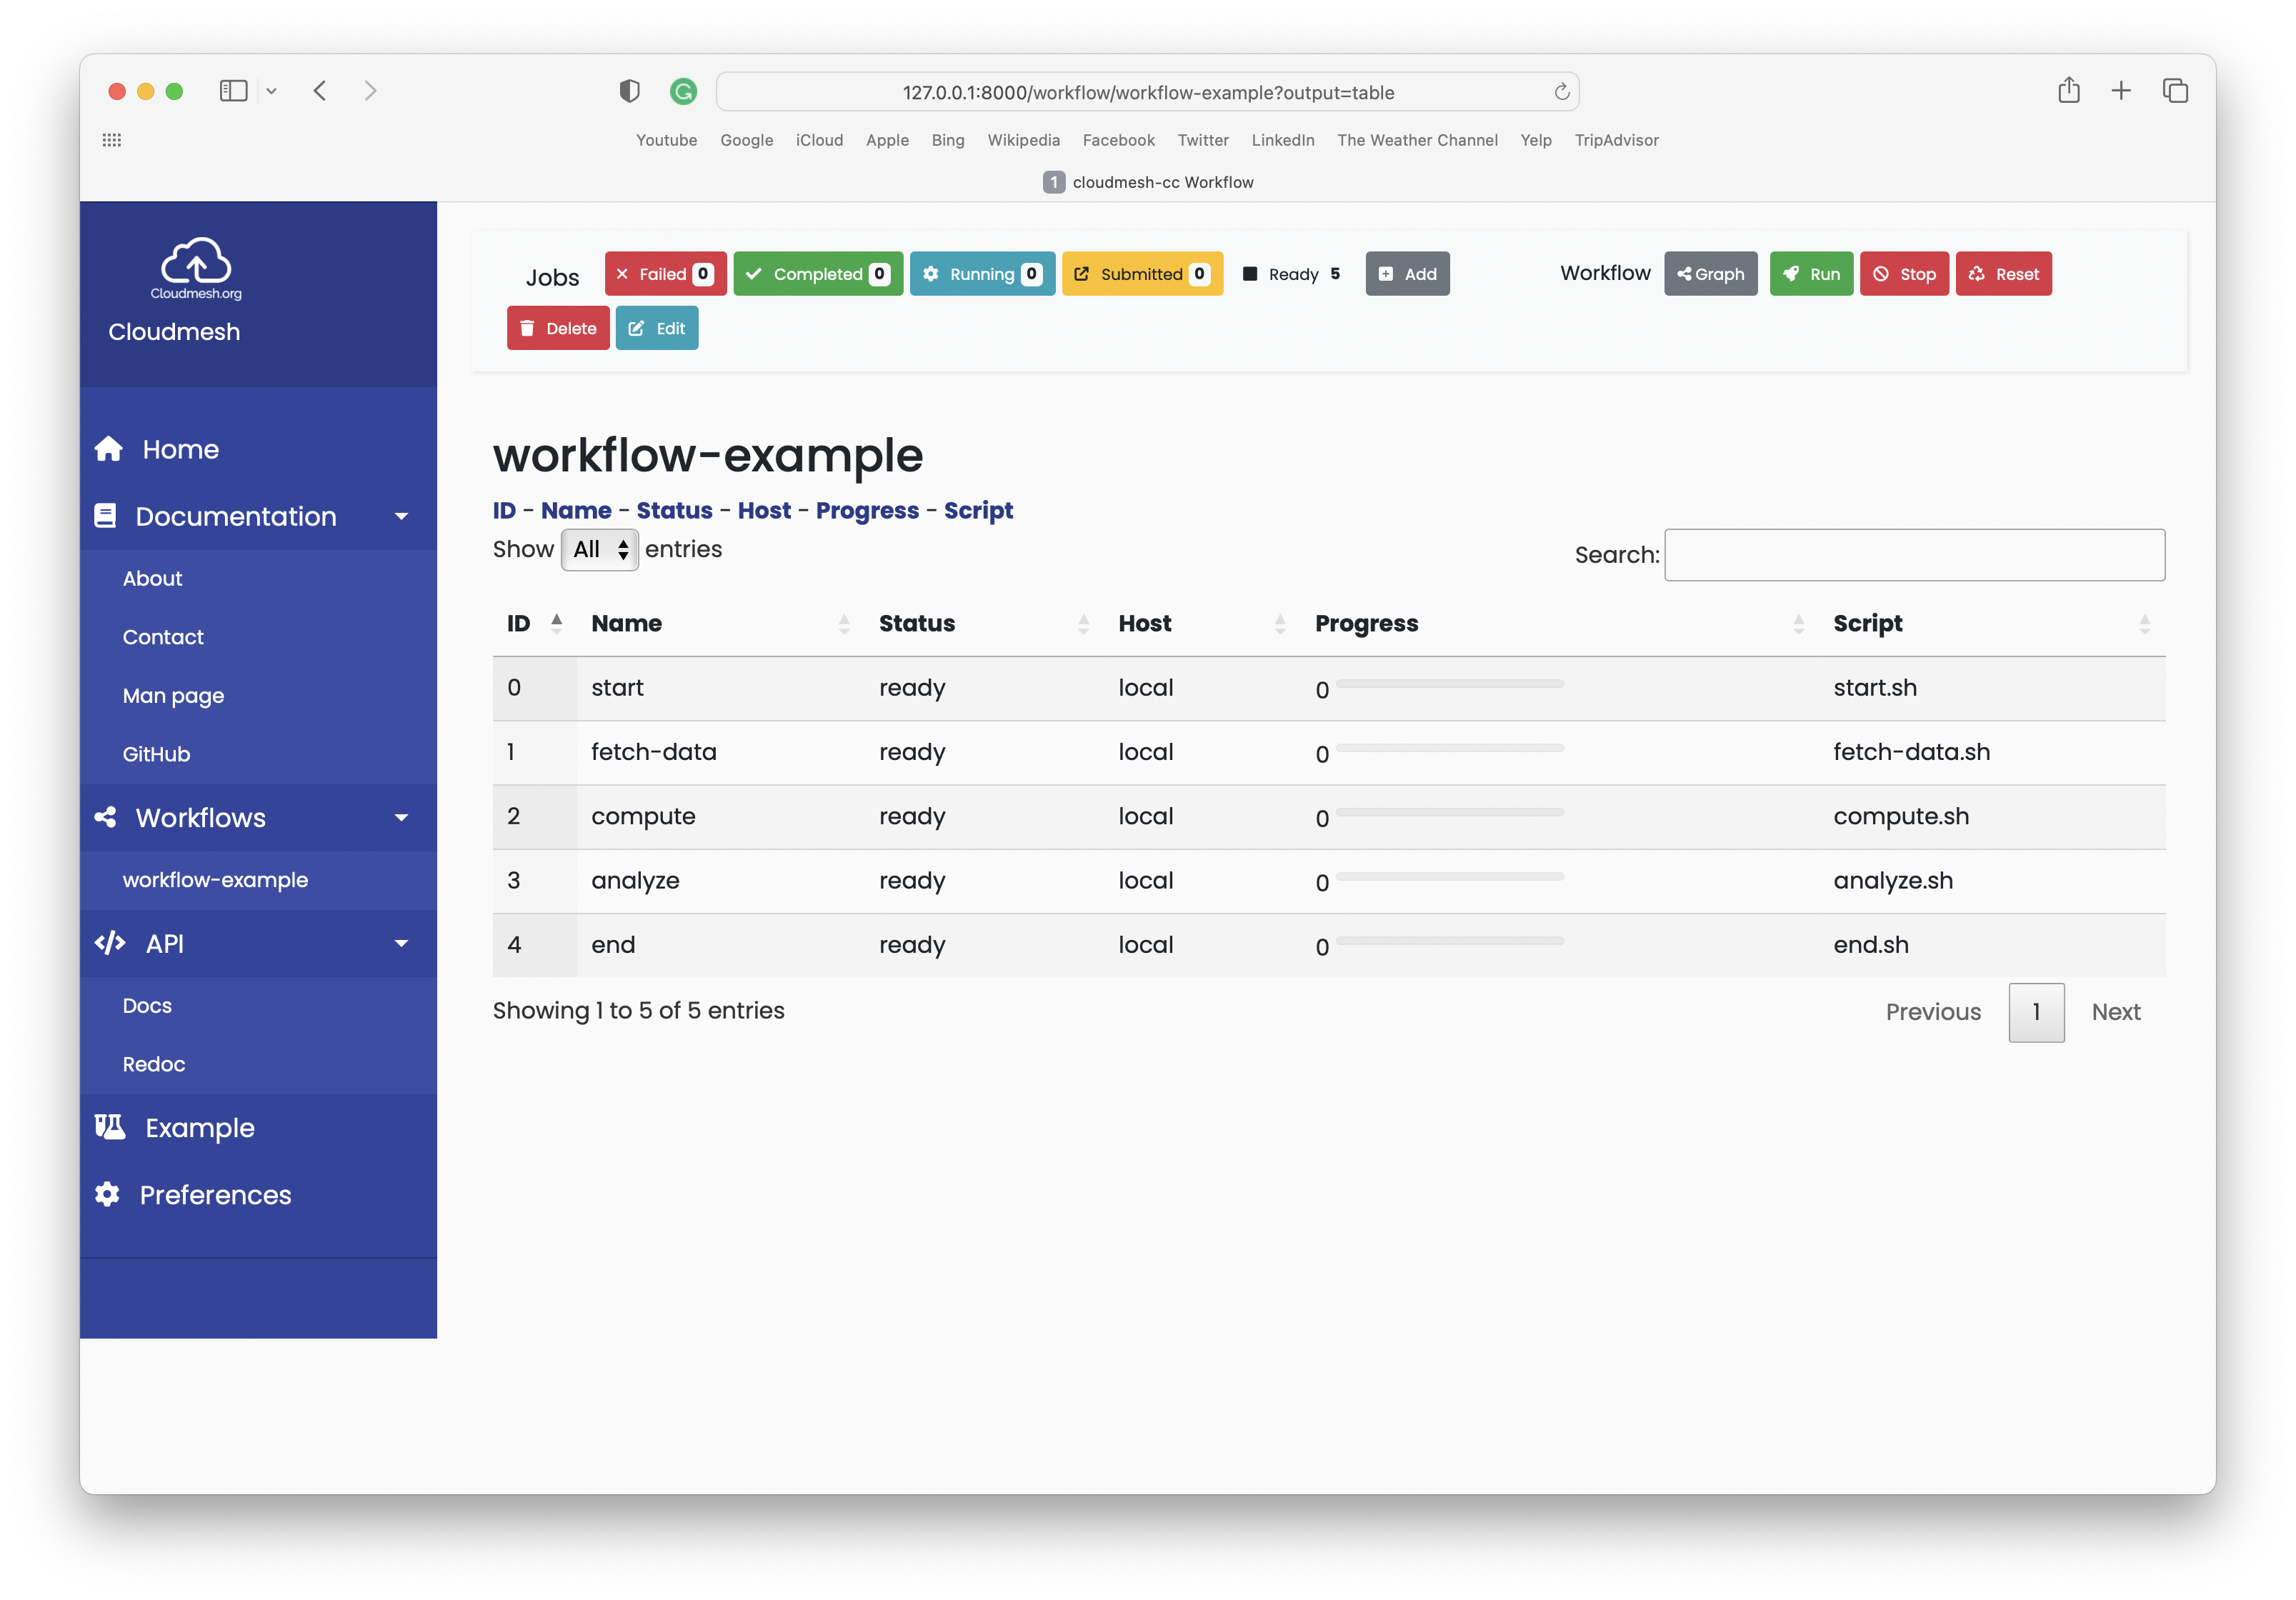
\includegraphics[width=1.05\columnwidth]{images/service-table.png}
\caption{Cloudmesh cc workflow Table view}
\end{figure}

\subsection{Graph View}\label{graph-view}

One can switch back and forth between a graph and a table view while
using the included buttons, it will take a moment to update them.

\begin{figure}
\centering
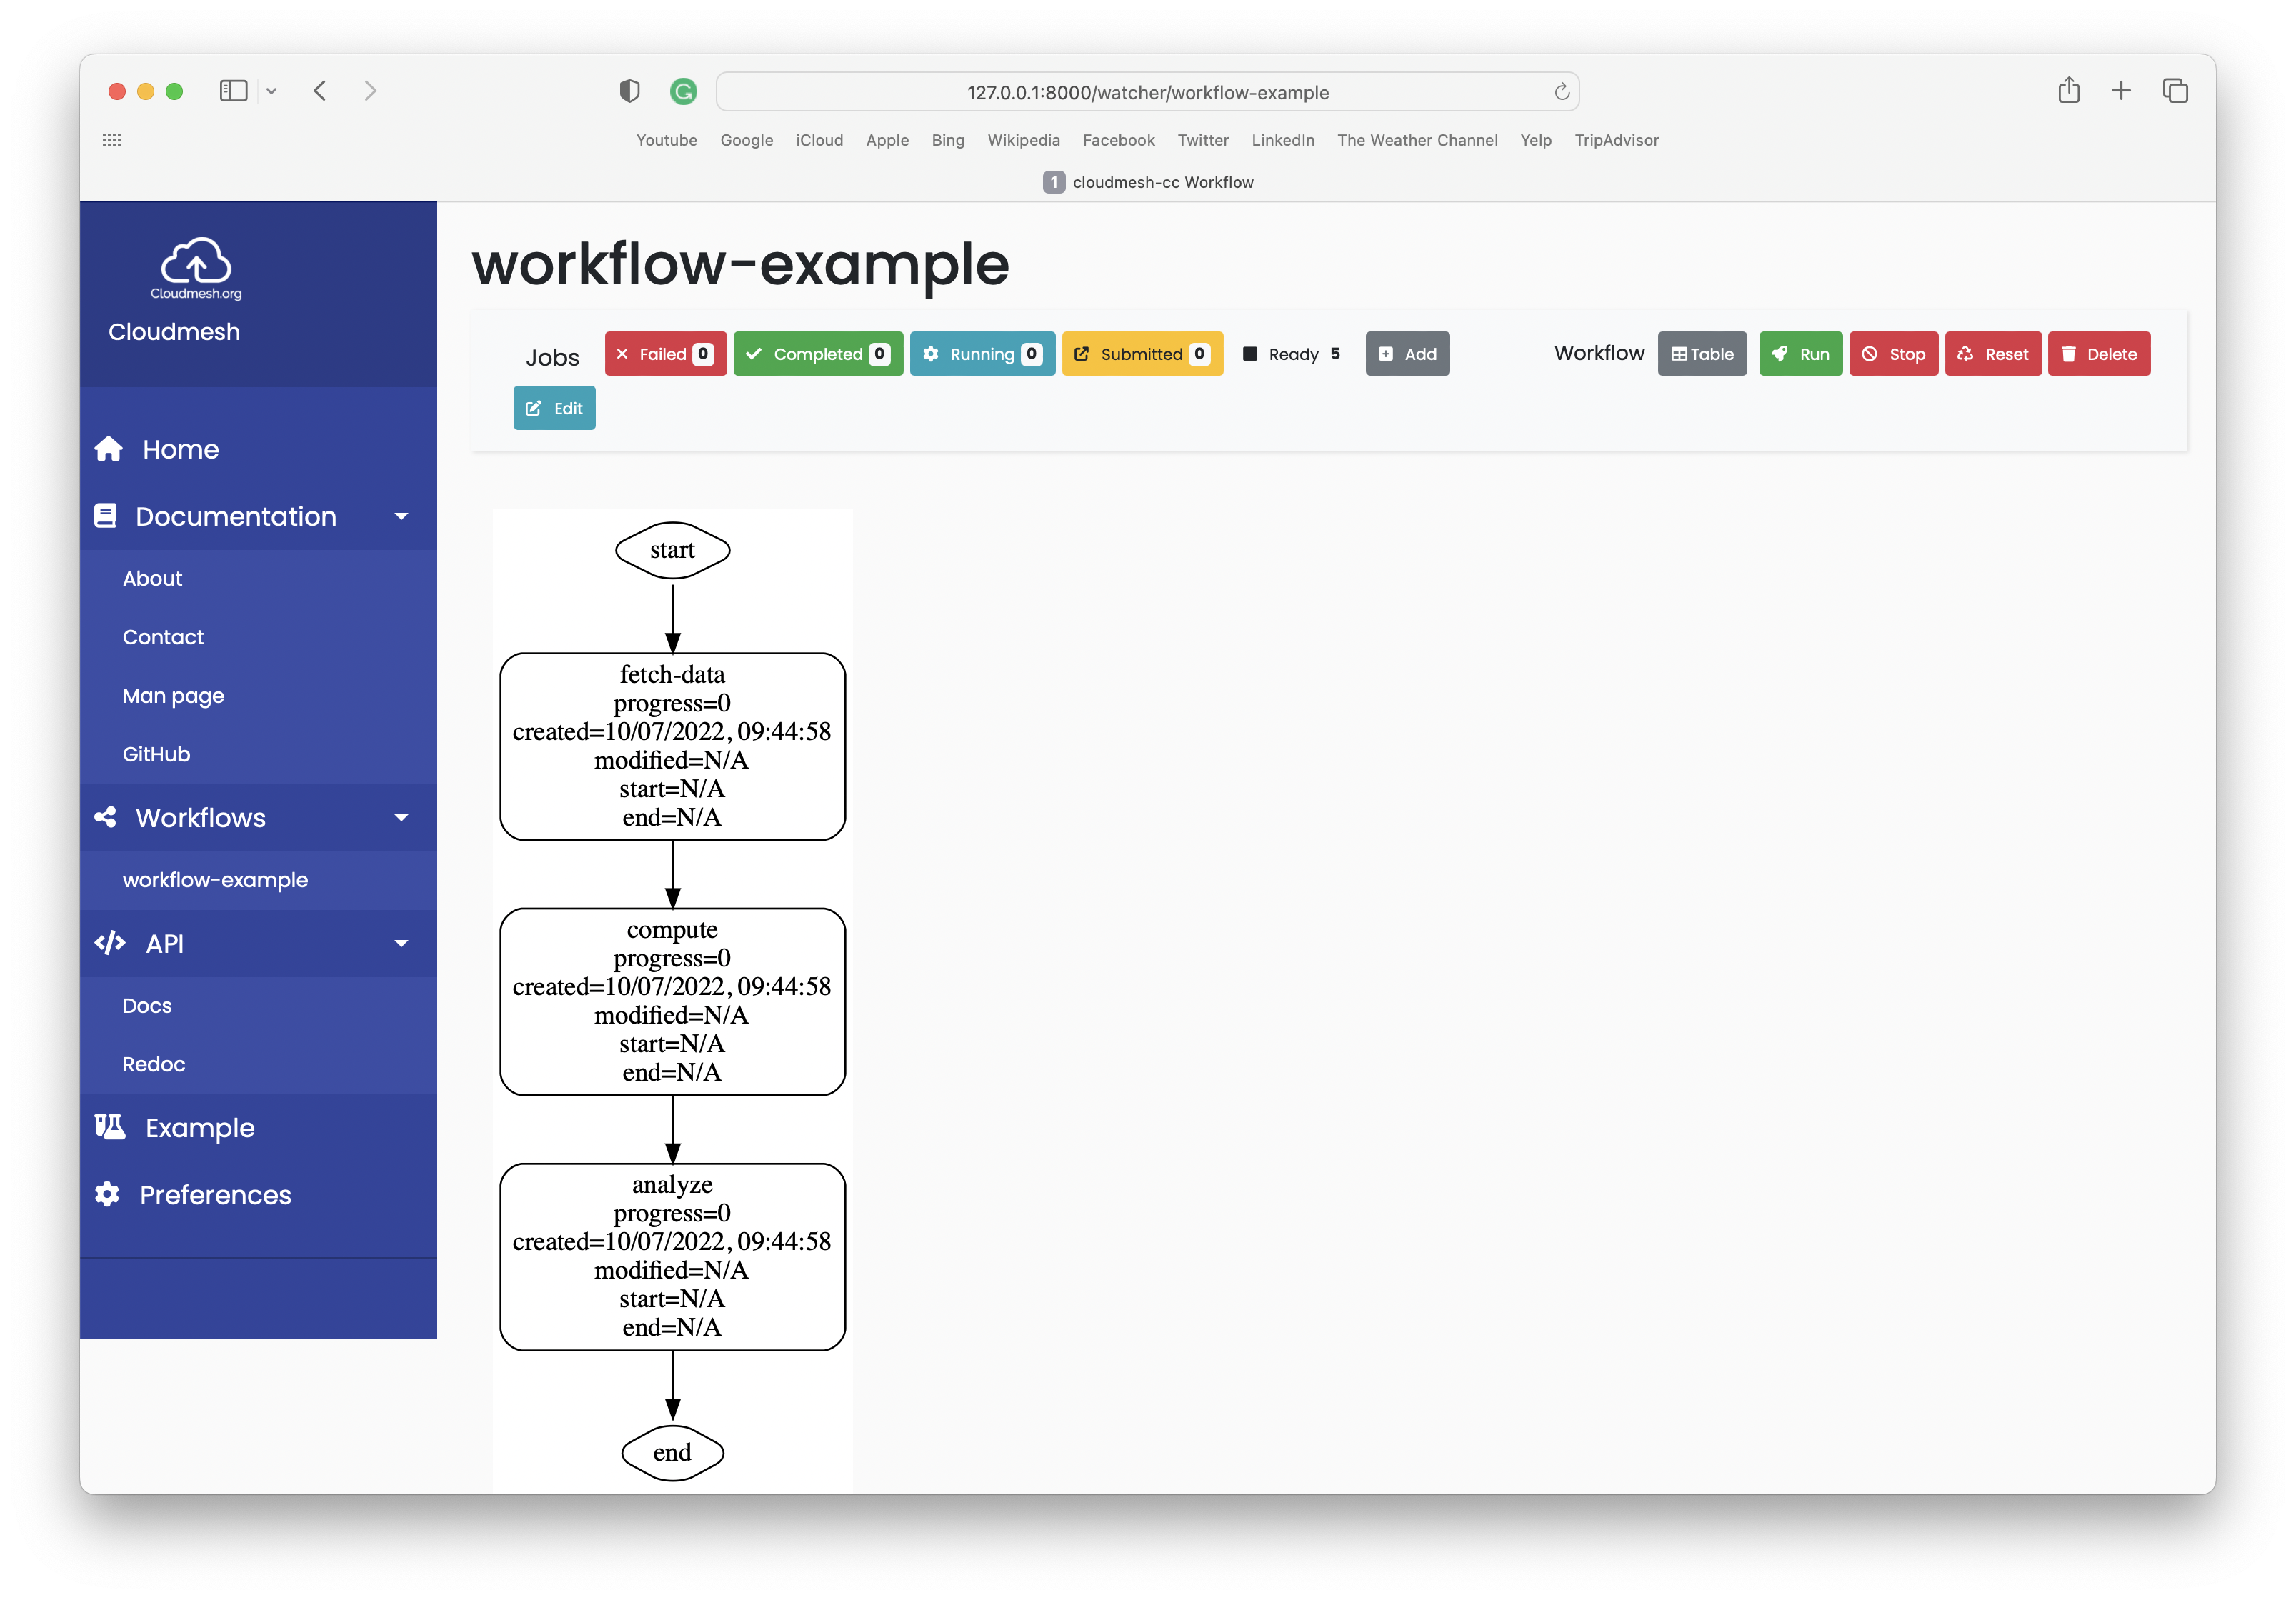
\includegraphics[width=1.05\columnwidth]{images/service-graph.png}
\caption{Cloudmesh cc workflow graph view}
\end{figure}

\section{Specifying Workflows}\label{specifying-workflows}

Users of cloudmesh cc must follow a certain configuration style to best
specify how a workflow should be run. Customization options include
specifying the job types, the order of how the jobs should be run, and
the portrayal of the graph.

\subsection{Workflow YAML format}\label{workflow-yaml-format}

A workflow yaml file with three Shell script jobs \texttt{a},
\texttt{b}, and \texttt{c} is as follows:

\begin{verbatim}
```text
workflow:
  nodes:
    a:
       name: a
       user: gregor
       host: localhost
       kind: local
       status: ready
       label: '{name}\nprogress={progress}'
       script: test-a.sh
    b:
       name: b
       user: gregor
       host: localhost
       kind: local
       status: ready
       label: '{name}\nprogress={progress}'
       script: test-b.sh
    c:
      name: c
      user: gregor
      host: localhost
      kind: local
      status: ready
      label: '{name}\nprogress={progress}'
      script: test-c.sh
  dependencies:
    - a,b,c
```
\end{verbatim}

\subsection{Example Workflows}\label{example-workflows}

Sample yaml files can be found at the following link:

\url{https://github.com/cloudmesh/cloudmesh-cc/blob/main/tests/workflow-example/workflow-example.yaml}

\subsection{Defining nodes in the
workflow}\label{defining-nodes-in-the-workflow}

Nodes can be customized in various ways within the workflow
configuration YAML file, including their job types (python, sh, jupyter,
or slurm), their virtual Python environment (by specifying
\texttt{venv}), their appearance on the graph, and other
characteristics.

\subsubsection{Defining labels for the
workflow}\label{defining-labels-for-the-workflow}

These variables must be in curly braces when defining the labels inside
the yaml workflow files.

For example, a label could be defined as follows:

\begin{verbatim}
```text
workflow:
  nodes:
    start:
      label: 'start\nCreated={created.%Y/%m/%d, %H--%M--%S}\nWorkflow Started={t0.%Y/%m/%d, %H--%M--%S}\nNow={now.%Y/%m/%d, %H--%M--%S}\nElapsed={dt0.%M--%S}'
```
\end{verbatim}

This creates a node on the graph that looks similar to the following
example:

\begin{figure}
\centering
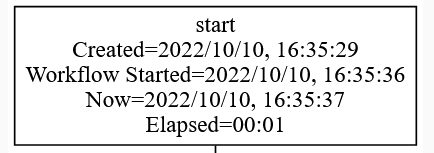
\includegraphics{images/labelmaker-example.png}
\caption{An example node with labels}
\end{figure}

Initially, the created and elapsed labels are \texttt{N/A} if the
workflow has not yet started, but they are replaced during runtime. This
can be observed by running a workflow in graph view in the web
interface.

Colons must be replaced with \texttt{-\/-} and the years, months, days,
hours, minutes, and seconds can be arranged as desired, as long as the
corresponding letters remain consistent (\texttt{\%Y} \texttt{\%m}
\texttt{\%d} \texttt{\%H} \texttt{\%M} \texttt{\%S} respectively). Also,
the format of the time must come immediately following the period.

\begin{itemize}
\tightlist
\item
  \texttt{name} name of job
\item
  \texttt{progress} progress of job from 0-100
\item
  time labels:

  \begin{itemize}
  \tightlist
  \item
    \texttt{now.} current time
  \item
    \texttt{now.\%Y/\%m/\%d,\ \%H-\/-\%M-\/-\%S} now in particular
    format (this can be used for other times as well)
  \item
    \texttt{created.} time when workflow was created
  \item
    \texttt{t0.} workflow start time
  \item
    \texttt{t1.} workflow end time
  \item
    \texttt{dt0.} elapsed time since workflow began
  \item
    \texttt{dt1.} total time of workflow once complete
  \item
    \texttt{tstart.} job start time
  \item
    \texttt{tend.} job end time
  \item
    \texttt{modified.} job modified time
  \end{itemize}
\item
  \texttt{os.} operating system environment variable (like os.HOME)
\item
  \texttt{cm.} cloudmesh variable that is read from \texttt{cms\ set}
\end{itemize}

\subsection{Defining format for timestamp
labels}\label{defining-format-for-timestamp-labels}

Various formats can be used for the timestamps, such as the American
datetime format \texttt{\%m/\%d/\%Y,\ \%H-\/-\%M-\/-\%S} or the
international datetime format \texttt{\%Y/\%m/\%d,\ \%H-\/-\%M-\/-\%S}.
As long as the letters stay consistent (\texttt{\%Y} \texttt{\%m}
\texttt{\%d} \texttt{\%H} \texttt{\%M} \texttt{\%S} for year, month,
day, hour, minute, and second, respectively), any format can be created.

If no format is specified following the period after the variable, the
datetime defaults to American format.

\subsection{Defining graphviz shapes and
styles}\label{defining-graphviz-shapes-and-styles}

Any shape and style for the nodes in the graph can be chosen, as long as
they are taken from the graphviz documentation:

\url{https://graphviz.org/doc/info/shapes.html}

\url{https://graphviz.org/docs/attr-types/style/}

The following is an example of a node in YAML format that uses a box
shape and an empty style. The empty style defaults to \texttt{filled},
which allows the node to change color when the job status is changed.

\begin{verbatim}
```text
workflow:
  nodes:
    start:
      label: 'start\nCreated={created.%Y/%m/%d, %H--%M--%S}\nWorkflow Started={t0.}\nElapsed={dt0.}'
      kind: local
      user: grey
      host: local
      status: ready
      exec: 'echo hello'
      name: start
      shape: box
      style: ''
```
\end{verbatim}

\subsection{Defining dependencies in the
workflow}\label{defining-dependencies-in-the-workflow}

Dependencies are specified in the order which jobs should be run, from
left to right. They are listed under the workflow in the yaml file.

\begin{verbatim}
```bash
workflow:
  nodes:
    a:
       name: a
    b:
       name: b
    c:
       name: c
  dependencies:
    - a,b,c
```
\end{verbatim}

\subsection{Reporting Progress}\label{reporting-progress}

When running scripts/jobs inside a workflow, the scripts must leverage
some format of cloudmesh.progress to run successfully. Otherwise, the
Workflow class cannot tell if the scripts are done, breaking the
progress functionality.

The examples that are provided with cloudmesh-cc are already augmented
with cloudmesh.progress. Thus, if a user is running self-made jobs and
workflows, they must adhere to the guidelines as follows.

\subsection{Shell and Slurm Scripts}\label{shell-and-slurm-scripts}

For shell and Slurm scripts \texttt{.sh}, the script must contain:

\begin{verbatim}
```bash
echo "# cloudmesh status=running progress=1 pid=$$"
```
\end{verbatim}

at the beginning of the script, and

\begin{verbatim}
```bash
echo "# cloudmesh status=done progress=100 pid=$$"
```
\end{verbatim}

at the end of the script.

\subsection{Python Scripts and Jupyter
Notebooks}\label{python-scripts-and-jupyter-notebooks}

For Python scripts \texttt{.py} and Jupyter notebooks \texttt{.ipynb},
the script must contain an import module from cloudmesh.common and calls
to the progress function.

py\_script.py

\begin{verbatim}
```bash
from cloudmesh.common.StopWatch import progress
from cloudmesh.common.Shell import Shell
filename = Shell.map_filename('./py_script.log').path
progress(progress=1, filename=filename)

# your script does what you want it to do here...

progress(progress=100, filename=filename)
```
\end{verbatim}

The statements do not need to be at the absolute beginning or end of the
script, but the progress must:

\begin{itemize}
\tightlist
\item
  be written to a filename with the same name as the script, ending in
  \texttt{.log}
\item
  begin at progress=1
\item
  and end at progress=100
\end{itemize}


\begin{acks}

  \FILE{acknowledgements.tex}

%\begin{ack}

\section*{Acknowledgements}

Continued work was in part funded by the NSF CyberTraining: CIC:
CyberTraining for Students and Technologies from Generation Z with the
award numbers 1829704 and 2200409 and NIST 60NANB21D151T. We like to
thank the students that participated in the REU for their help and
evaluation in a pre-alpha version of the code. We are excited that
this effort contributed significantly to their increased understanding
of Python and how to develop in a team using the Python ecosystem.

%\end{ack}


\end{acks}

\bibliographystyle{ACM-Reference-Format}
\bibliography{references}


\usepackage{appendix}

\section{Contributing}\label{contributing}

\subsection{GitHub}\label{github}

The code is maintained on GitHub

\begin{itemize}
\tightlist
\item
  \href{https://github.com/cloudmesh/cloudmesh-cc}{Code}
\item
  \href{https://github.com/cloudmesh/cloudmesh-cc/issues}{Issues}
\item
  \href{https://github.com/cloudmesh/cloudmesh-cc/pulls}{Pull Requests}
\item
  \href{https://github.com/cloudmesh/cloudmesh-cc/actions}{Actions}
\item
  \href{https://github.com/cloudmesh/cloudmesh-cc/pulse}{Insights}
\end{itemize}

The code was developed by Gregor von Laszewski and J.P. Fleischer. Other
contributors to a pre alpha version are listed at

\begin{itemize}
\tightlist
\item
  \href{https://github.com/cloudmesh/cloudmesh-cc/graphs/contributors}{Contributors}
\end{itemize}

\subsection{Management}\label{management}

All contributions will be done under the apache license. The code will
be managed in open-source. Pull requests need to be made in the
repository. The main branch is the release branch. Contributions will
first be done in other branches, and once we agree that they need to be
integrated into the code, they will be merged into main. All new code
must have sufficient pytests. The pytests may need to be documented in
case special authentication is required.

We follow a
\href{https://docs.github.com/en/get-started/quickstart/github-flow}{typical
GitHub workflow} of:

\begin{itemize}
\tightlist
\item
  create a personal fork of this repo
\item
  create a branch
\item
  open a pull request
\item
  fix findings of various linters and checks
\item
  work through code review
\end{itemize}

For each pull request, the documentation is built and deployed to make
it easier to review the changes in the pull request.

\hypertarget{tests}{%
\subsection{Tests}\label{tests}}

Before creating a pull request it is important that the tests in the
test directory pass.

The tests are organized as follows:

\begin{itemize}
\tightlist
\item
  \texttt{pytest\ tests/test\_0??\_*} will run locally and only use
  ascii output
\item
  \texttt{pytest\ tests/test\_1??\_*} will run locally but also present
  graphs
\end{itemize}

in future we will likely change this and allow a test variable
\texttt{cms\ set\ test\_with\_graph=False/True} and if it is not
existent it is False. In case it is false the graohs will not be
displayed. but the test will be run. This change will also allow tests
with 1?? to be run on github workflows

\begin{itemize}
\tightlist
\item
  \texttt{pytest\ tests/test\_5??\_*} will run on remote machines and
  require at this time rivanna from UVA
\end{itemize}

in future this test will be modified so we can specify the remote user
and remote host \texttt{cms\ set\ test\_remote\_user=TBD}
\texttt{cms\ set\ test\_remote\_host=TBD}. If they do not exist they
will use the defualts from ssh config rivanna. verify if logic is ok.

\begin{itemize}
\tightlist
\item
  \texttt{pytest\ tests/test\_6??\_*} will test the rest service
\item
  \texttt{pytest\ tests/test\_9??\_*} will cleanup the tests
\end{itemize}

\FILE{installation.tex}

\section{Installation}\label{installation}

To leverage cloudmesh-cc, use the cloudmesh-installer to install the
Cloudmesh suite of repositories. Optionally, to utilize the graph
visualization you must install also {\em graphviz} must be
installed. On Windows, Git Bash is required, in addition.  The overall
installation is very simple and is supported on a variety of operating
systems.  We leverage the cloudmesh-installer to locally install the
cloudmesh suite of repositories by executing the following commands:

\begin{minted}[breaklines]{bash}
$ mkdir ~/cm
$ cd ~/cm
$ pip install cloudmesh-installer -U
$ cloudmesh-installer get cc
\end{minted}

To install graphviz you can use the following commands on the appropriate operating system:

\begin{description}

\item[Windows.]
Git Bash and Graphviz must be installed. The user can use Chocolatey to run
as an administrator for convenience:

\begin{minted}[breaklines]{bash}
$ choco install git.install --params "/GitAndUnixToolsOnPath /Editor:Nano /PseudoConsoleSupport /NoAutoCrlf" -y
$ choco install graphviz -y
\end{minted}

\item[macOS.] Graphviz must be installed. The user can use Homebrew for convenience:

\begin{minted}[breaklines]{bash}
$ brew install graphviz
\end{minted}

\item[Linux.] Graphviz must be installed. The user can use apt for convenience:

\begin{minted}[breaklines]{bash}
$ sudo apt install graphviz -y
\end{minted}

\end{description}

To test the workflow program, prepare a cm directory in your home
directory by executing the following commands:

\begin{minted}[breaklines]{bash}
$ cd ~/cm/cloudmesh-cc
$ pytest -v -x --capture=no tests
\end{minted}

A variety of separate tests are available that test individual capabilities. 




\end{document}
\endinput
%%
%% End of file `sample-sigplan.tex'.
